Table~\ref{tab:main-results} reports test mAP@0.5 for every (method, budget) cell, averaged over three seeds, with the per-seed range in brackets. Figure~\ref{fig:sample-eff} plots the same data as sample-efficiency curves, with seed range shown as asymmetric error bars. Three observations stand out.

% Auto-generated by scripts/build_paper_assets.py — do not edit by hand.
\begin{table}[t]
\centering
\small
\caption{Held-out kiwi test mAP@0.5 by method and label budget. Each cell is the mean over three seeds (42, 43, 44); the bracketed range is [min, max]. Bold marks the best mean per column.}
\label{tab:main-results}
\begin{tabular}{lrrrrr}
\toprule
Method & $n{=}10$ & $n{=}25$ & $n{=}50$ & $n{=}100$ & $n{=}181$ \\
\midrule
Scratch & 0.002~[0.000,\,0.005] & 0.004~[0.000,\,0.009] & 0.237~[0.000,\,0.699] & 0.881~[0.866,\,0.893] & 0.906~[0.897,\,0.914] \\
COCO transfer & 0.362~[0.065,\,0.687] & \textbf{0.892}~[0.871,\,0.914] & \textbf{0.925}~[0.921,\,0.931] & \textbf{0.940}~[0.934,\,0.947] & \textbf{0.940}~[0.937,\,0.944] \\
CrossPoll (full FT) & 0.454~[0.408,\,0.539] & 0.390~[0.335,\,0.481] & 0.908~[0.902,\,0.914] & 0.919~[0.914,\,0.921] & 0.926~[0.925,\,0.927] \\
CrossPoll + freeze & \textbf{0.630}~[0.591,\,0.672] & 0.871~[0.867,\,0.877] & 0.889~[0.883,\,0.892] & 0.909~[0.905,\,0.913] & 0.922~[0.921,\,0.923] \\
\bottomrule
\end{tabular}
\end{table}


\begin{figure}[t]
  \centering
  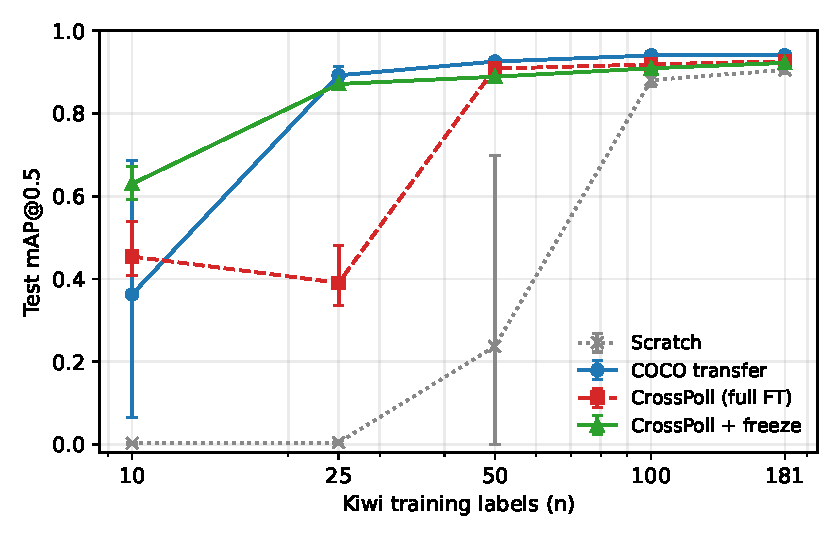
\includegraphics[width=\linewidth]{figures/sample_efficiency.pdf}
  \caption{Test mAP@0.5 on the held-out kiwi crop as a function of the number of fine-tuning labels. Markers show the mean over three seeds; error bars span the per-seed range. The x-axis is logarithmic. Backbone freezing rescues CrossPoll at the smallest budgets and produces the most stable curve overall, while COCO transfer keeps a small lead from $n{=}50$ onward.}
  \label{fig:sample-eff}
\end{figure}

\paragraph{Backbone freezing rescues the small-budget collapse.} Without freezing, CrossPoll fine-tuning at $n{=}25$ produces a mean mAP@0.5 of 0.390 with all three seeds in the range [0.335, 0.481]. Inspection of the per-epoch training logs (under \texttt{runs/step3/crosspoll/}) shows a consistent failure mode across seeds: validation mAP peaks at epoch 3 and then deteriorates monotonically until early stopping fires at epoch 18. With \texttt{freeze=10} applied --- and patience extended from 15 to 30 epochs to give the head more time to settle --- the same configuration achieves 0.871 [0.867, 0.877], a 48-point absolute increase that brings CrossPoll within two points of COCO transfer at the same budget.

\paragraph{CrossPoll with freezing dominates the extreme few-shot regime.} At $n{=}10$, CrossPoll + freeze attains a mean of 0.630 with a tight range of [0.591, 0.672]. COCO transfer at the same budget averages 0.362 but spreads across [0.065, 0.687] --- one of the three seeds essentially fails to converge. The from-scratch baseline produces near-zero mAP at this budget for all seeds, as expected. The variance gap is as relevant as the mean gap for a deployment context: a robotic pollination pipeline that needs to add a new crop can tolerate a small absolute accuracy drop, but a one-in-three chance of complete failure is much harder to manage operationally.

\paragraph{COCO transfer leads at moderate to higher budgets.} From $n{=}50$ upward, COCO transfer's mean mAP@0.5 (0.926, 0.940, 0.940) edges out both CrossPoll variants by roughly one to three absolute points. The full-fine-tune CrossPoll variant catches up faster than the frozen one, ending at 0.927 at $n{=}181$ versus 0.922 for the frozen variant. Backbone freezing therefore appears to act as a constraint that pays its largest dividends at very small budgets and exacts a small but consistent cost once enough labels are available for full fine-tuning to converge cleanly. The from-scratch baseline reaches a competitive 0.906 at $n{=}181$, confirming that with enough labels the choice of pretrain matters less.

\paragraph{Stricter mAP@0.5{:}0.95.} Where logged, the secondary metric tracks the headline mAP@0.5 trends but with a smaller absolute gap between methods. At $n{=}181$ COCO transfer scores 0.642, CrossPoll (full FT) scores 0.628, and CrossPoll + freeze scores 0.604. Domain-matched pretraining does not yield tighter bounding boxes than COCO at this kiwi test set; the test set's small size (61 images) and the YOLOv8n backbone's limited regression capacity together appear to cap the achievable mAP@0.5{:}0.95 around 0.65 for any of the methods we evaluated.
